%==============================================================================
% Paper Research Methods: onderzoeksvoorstel
%==============================================================================

\documentclass{hogent-article}

\usepackage{lipsum} % Voor vultekst

% Invoegen bibliografiebestand
\usepackage[backend=biber,style=apa]{biblatex}
\DeclareLanguageMapping{dutch}{dutch-apa}
\addbibresource{references.bib}

% Informatie over de opleiding, het vak en soort opdracht
\studyprogramme{Professionele bachelor toegepaste informatica}
\course{Research Methods}
\assignmenttype{Paper: Onderzoeksvoorstel}
\academicyear{2023-2024}



\title{Gamification voor milieu- en duurzaamheidsinitiatieven in een gemeente}


\author{Präben Bryse}
\email{praben.bryse@student.hogent.be}


% TODO (fase 1): Geef hier de link naar jullie Github-repository
\projectrepo{https://github.com/pbryse/RMBryseP}

% Binnen welke specialisatierichting uit 3TI situeert dit onderzoek zich?
% Kies uit deze lijst:
%
% - Mobile \& Enterprise development
% - AI \& Data Engineering
% - Functional \& Business Analysis
% - System \& Network Administrator
% - Mainframe Expert
% - Als het onderzoek niet past binnen een van deze domeinen specifieer je deze
%   zelf
%
\specialisation{Mobile \& Enterprise development}
% Geef hier enkele sleutelwoorden die je onderwerp beschrijven
\keywords{Gamification, Milieu, Duurzaamheid, Gemeente, Gedragsverandering}

\begin{document}
    
\begin{abstract}
    In de huidige maatschappij wordt duurzaamheid een steeds grotere zorg voor gemeenten. Zij staan voor de uitdaging om hun inwoners meer te betrekken bij milieu- en duurzaamheidsinitiatieven. Deze studie onderzoekt hoe de toepassingen van gamification kunnen worden ingezet om de betrokkenheid te vergroten en duurzaam gedrag te verkrijgen binnen een gemeente. Door spelelementen zoals punten, badges en klassementen toe te passen, heeft dit onderzoek als doel een \emph{gamified platform} te ontwikkelen en te testen in een fictieve gemeente Zonnedorp. De verwachte resultaten zeggen dat gamification niet alleen de betrokkenheid van de inwoners bij de reeds bestaande initiatieven zal verhogen, maar ook zal leiden tot verbetering in duurzaam gedrag. Dit onderzoek zal uiteindelijk resulteren in een Proof-of-Concept, samen met aanbevelingen voor de verdere ontwikkeling. 
\end{abstract}

\tableofcontents

\bigskip

%
\paragraph{Door langdurige afwezigheid heb ik niets kunnen indienen voor EP2.}
%
% Beschrijf hier kort de verschillen en/of verbeteringen t.o.v. je originele
% voorstel.

\section{Inleiding}%
\label{sec:inleiding}

In een tijdperk waarin duurzaamheid steeds belangrijker wordt, staan gemeenten voor de uitdaging om hun burgers actief te betrekken bij milieuvriendelijke initiatieven. Ondanks de vele initiatieven die zijn opgezet om duurzaam gedrag te verkrijgen, blijft de betrokkenheid en actieve deelname van burgers de grootste uitdaging. 

\emph{Gamification}, het toepassen van spelelementen in een niet-spelcontext, biedt een nieuwe manier aan om deze uitdaging aan te pakken door het stimuleren van gedragsverandering en betrokkenheid.

Dit onderzoek richt zich op de toepassing van gamification in een gemeentelijke omgeving, specifiek gericht op het verbeteren van milieubewustzijn en duurzaam gedrag bij de inwoners. Gamification maakt gebruik van spelelementen zoals punten, badges, uitdagingen en ranglijsten om gebruikers te motiveren en betrokken te houden.

\textbf{Omdat dit een fictieve casus is, wordt de gemeente Zonnedorp gekozen. Deze gemeente bestaat niet, maar dient als richtlijn. Indien dit onderzoek volledig wordt uitgewerkt, zal een bestaande gemeente gekozen moeten worden, waarbij het onderzoek specifiek voor die gemeente verder ontwikkeld kan worden.} 

De gemeente Zonnedorp heeft reeds bestaande initiatieven en pogingen ondernomen zoals buurtmoestuinen waar inwoners hun eigen groenten en fruit kunnen kweken, deelauto's en deelfietsen ter beschikking gesteld en een jaarlijkse duurzaamheidsbeurs opgericht waar duurzame producten en diensten getoond worden. Echter hebben deze traditionele methodes en prikkels niet het gewenste effect gehad. 

De centrale onderzoeksvraag van deze bachelorproef luidt daarom: 

\textbf{Hoe kan gamification worden ingezet om de betrokkenheid van burgers bij milieu- en duurzaamheidsinitiatieven in de gemeente Zonnedorp te vergroten en meetbare verbeteringen te realiseren in milieuvriendelijk gedrag?}

Het doel van dit onderzoek is om een gamified platform te ontwikkelen en te testen of de betrokkenheid van de inwoners van Zonnedorp bij duurzaamheidsinitiatieven vergroot.

Het eindresultaat van dit onderzoek zal een proof-of-concept van het platform zijn, samen met een evaluatierapport met aanbevelingen voor verdere optimalisatie. Het onderzoek is succesvol als het platform een significante verbetering laat zien in de betrokkenheid van inwoners bij milieuvriendelijke initiatieven.

\section{Literatuurstudie}%
\label{sec:literatuurstudie}
\subsection{Gamification?}
\subsubsection{Wat is gamification?}
Gamification is het gebruik van game-ontwerp-elementen, zoals punten, badges en klassementen, in niet-game contexten. \autocite{Deterding2011} \textcite{Burke2016} beschrijft gamification als een krachtig instrument om gebruikers te motiveren door het stimuleren van gedragsverandering via beloningssystemen.

Er zijn verschillende soorten elementen die gebruikt kunnen worden:
\begin{itemize}
    \item \textbf{Puntensysteem:} hierbij worden punten uitgedeeld voor het uitvoeren van verschillende taken \autocite{Kondrat2024}
    \item  \textbf{Badges:} badges worden toegekend als je een bepaalde grenswaarde van iets bereikt hebt (10 posts gemaakt op een blogsite, voor de eerste keer 5km gelopen,...) \autocite{Kondrat2024}
    \item \textbf{Queestes:} een queeste verwijst naar een specifieke taak of reeks van taken die deelnemers moeten voltooien om een bepaald doel te bereiken. Vaak zijn queestes  opgedeeld in kleinere missies die leiden tot het voltooien van een grotere taak. \autocite{Wanasek2023}
    \item \textbf{Klassementen:} klassementen tonen de rangorde van gebruikers op basis van hun verzamelde punten of prestaties, waardoor een (gezonde) competitieve omgeving gecreëerd wordt. Dit stimuleert gebruikers om beter te presteren en hoger op de ranglijst te komen. \autocite{Werbach2012}
    \item \textbf{Levels:} het gebruik van levels helpt gebruikers om hun voortgang te meten en biedt een gevoel van groei en ontwikkeling naarmate ze meer ervaring opdoen. \autocite{Werbach2012}
    \item \textbf{Feedbacksystemen:} gamification maakt vaak gebruik van directe feedbacksystemen zoals meldingen of voortgangsbalken, om de gebruikers te informeren over hun prestaties en wat ze kunnen doen om verder te komen \autocite{Deterding2011}
\end{itemize}

\subsubsection{Hoe werkt gamification}

De belangrijkste reden waarom gamification werkt, is omdat het gebaseerd is op het psychologische mechanisme van intrinsieke motivatie zoals de behoeften aan autonomie, competentie en sociale verbondenheid. \autocite{Ryan2000}

Gamification maakt gebruik van gedragsmodellen zoals het Fogg Behavior Model (FBM) dat zegt dat drie elementen op hetzelfde moment moeten samenkomen om een ​​gedrag te laten optreden: motivatie, capaciteit en een trigger. Wanneer een gedrag niet optreedt, ontbreekt ten minste één van die elementen. \autocite{Fogg_2009}

Hoewel gamification vaak gezien wordt als een middel om het engagement op korte termijn te doen toenemen, zegt onderzoek ook dat het een invloed heeft op lange termijn. Zelfs wanneer de spelelementen weg gehaald worden, is er een duidelijke gedragsverandering merkbaar. Het engagement is wel afgenomen eens de spelelementen weg waren, maar was wel significant beter dan helemaal in het begin van het onderzoek. \autocite{Li_2024}

\subsection{Gamification en duurzaamheid}
Er zijn een aantal studies gebeurd naar het gebruik van gamification om meer duurzaam gedrag te verkrijgen. 

Zo zegt de studie van \textcite{Hassan_2020} dat \textit{gamified e-participatie} gekoppeld is aan verhoogde betrokkenheid, motivatie, burgerlijk leren en plezier.

Ook \textcite{McConigal2011} benadrukt het potentieel van \emph{games} om complexe problemen op te lossen, waaronder milieuproblemen.

\subsection{Uitdagingen}
Hoewel gamification veelbelovend is, zijn er ook uitdagingen. Onderzoekers waarschuwen voor de mogelijke negatieve effecten, zoals overmatige afhankelijkheid van extrinsieke beloningen, wat de intrinsieke motivatie kan ondermijnen. \autocite{Buznea2021}


\section{Methodologie}%
\label{sec:methodologie}

In de eerste fase, de opstartfase, is er tijd vrijgemaakt voor het verder verdiepen van de literatuur studie. Daarnaast zal er ook een planning gemaakt worden. Deze fase duurt ongeveer twee weken.

In de tweede fase ligt de focus op het verzamelen van de functionele en niet-functionele requirements. Hiervoor wordt met de copromoter, die werkt voor de gemeente Zonnedorp, samen gezeten om de evaluatiecriteria op te stellen. Vervolgens worden de requirements ingedeeld via de MoSCoW-methode. Elke requirement krijgt een een van de volgende labels: \emph{must have, should have, could have} of \emph{won't have.} Hierdoor krijgen we een goed overzicht van de requirements gegroepeerd op hun prioriteit.

Verder, in de derde fase,  wordt de \emph{Proof-of-Concept} (PoC) uitgewerkt. Eerst wordt er bepaald welke gamifi-catie-elementen gebruikt zullen worden. Op basis van die gekozen elementen zullen de evaluatiecriteria bepaald worden.

Nadien wordt de applicatie uitgewerkt samen met de gamificatie-elementen. Het is belangrijk om die elementen modulair te maken zodat ze gemakkelijk uit het project gelaten kunnen worden en eventueel andere toegevoegd worden. Zo kunnen we in een latere fase, de pilot fase, twee groepen creëren om eenvoudig \emph{A/B testing} te hanteren.

In deze fase zal er \emph{agile} gewerkt worden, met sprints van twee weken. Hierbij zal er op het einde van de sprint steeds samen gezeten worden met de gemeente Zonnedorp om onmiddellijk feedback te hebben. Deze fase duurt zes weken. 

\begin{figure*}
    \centering
    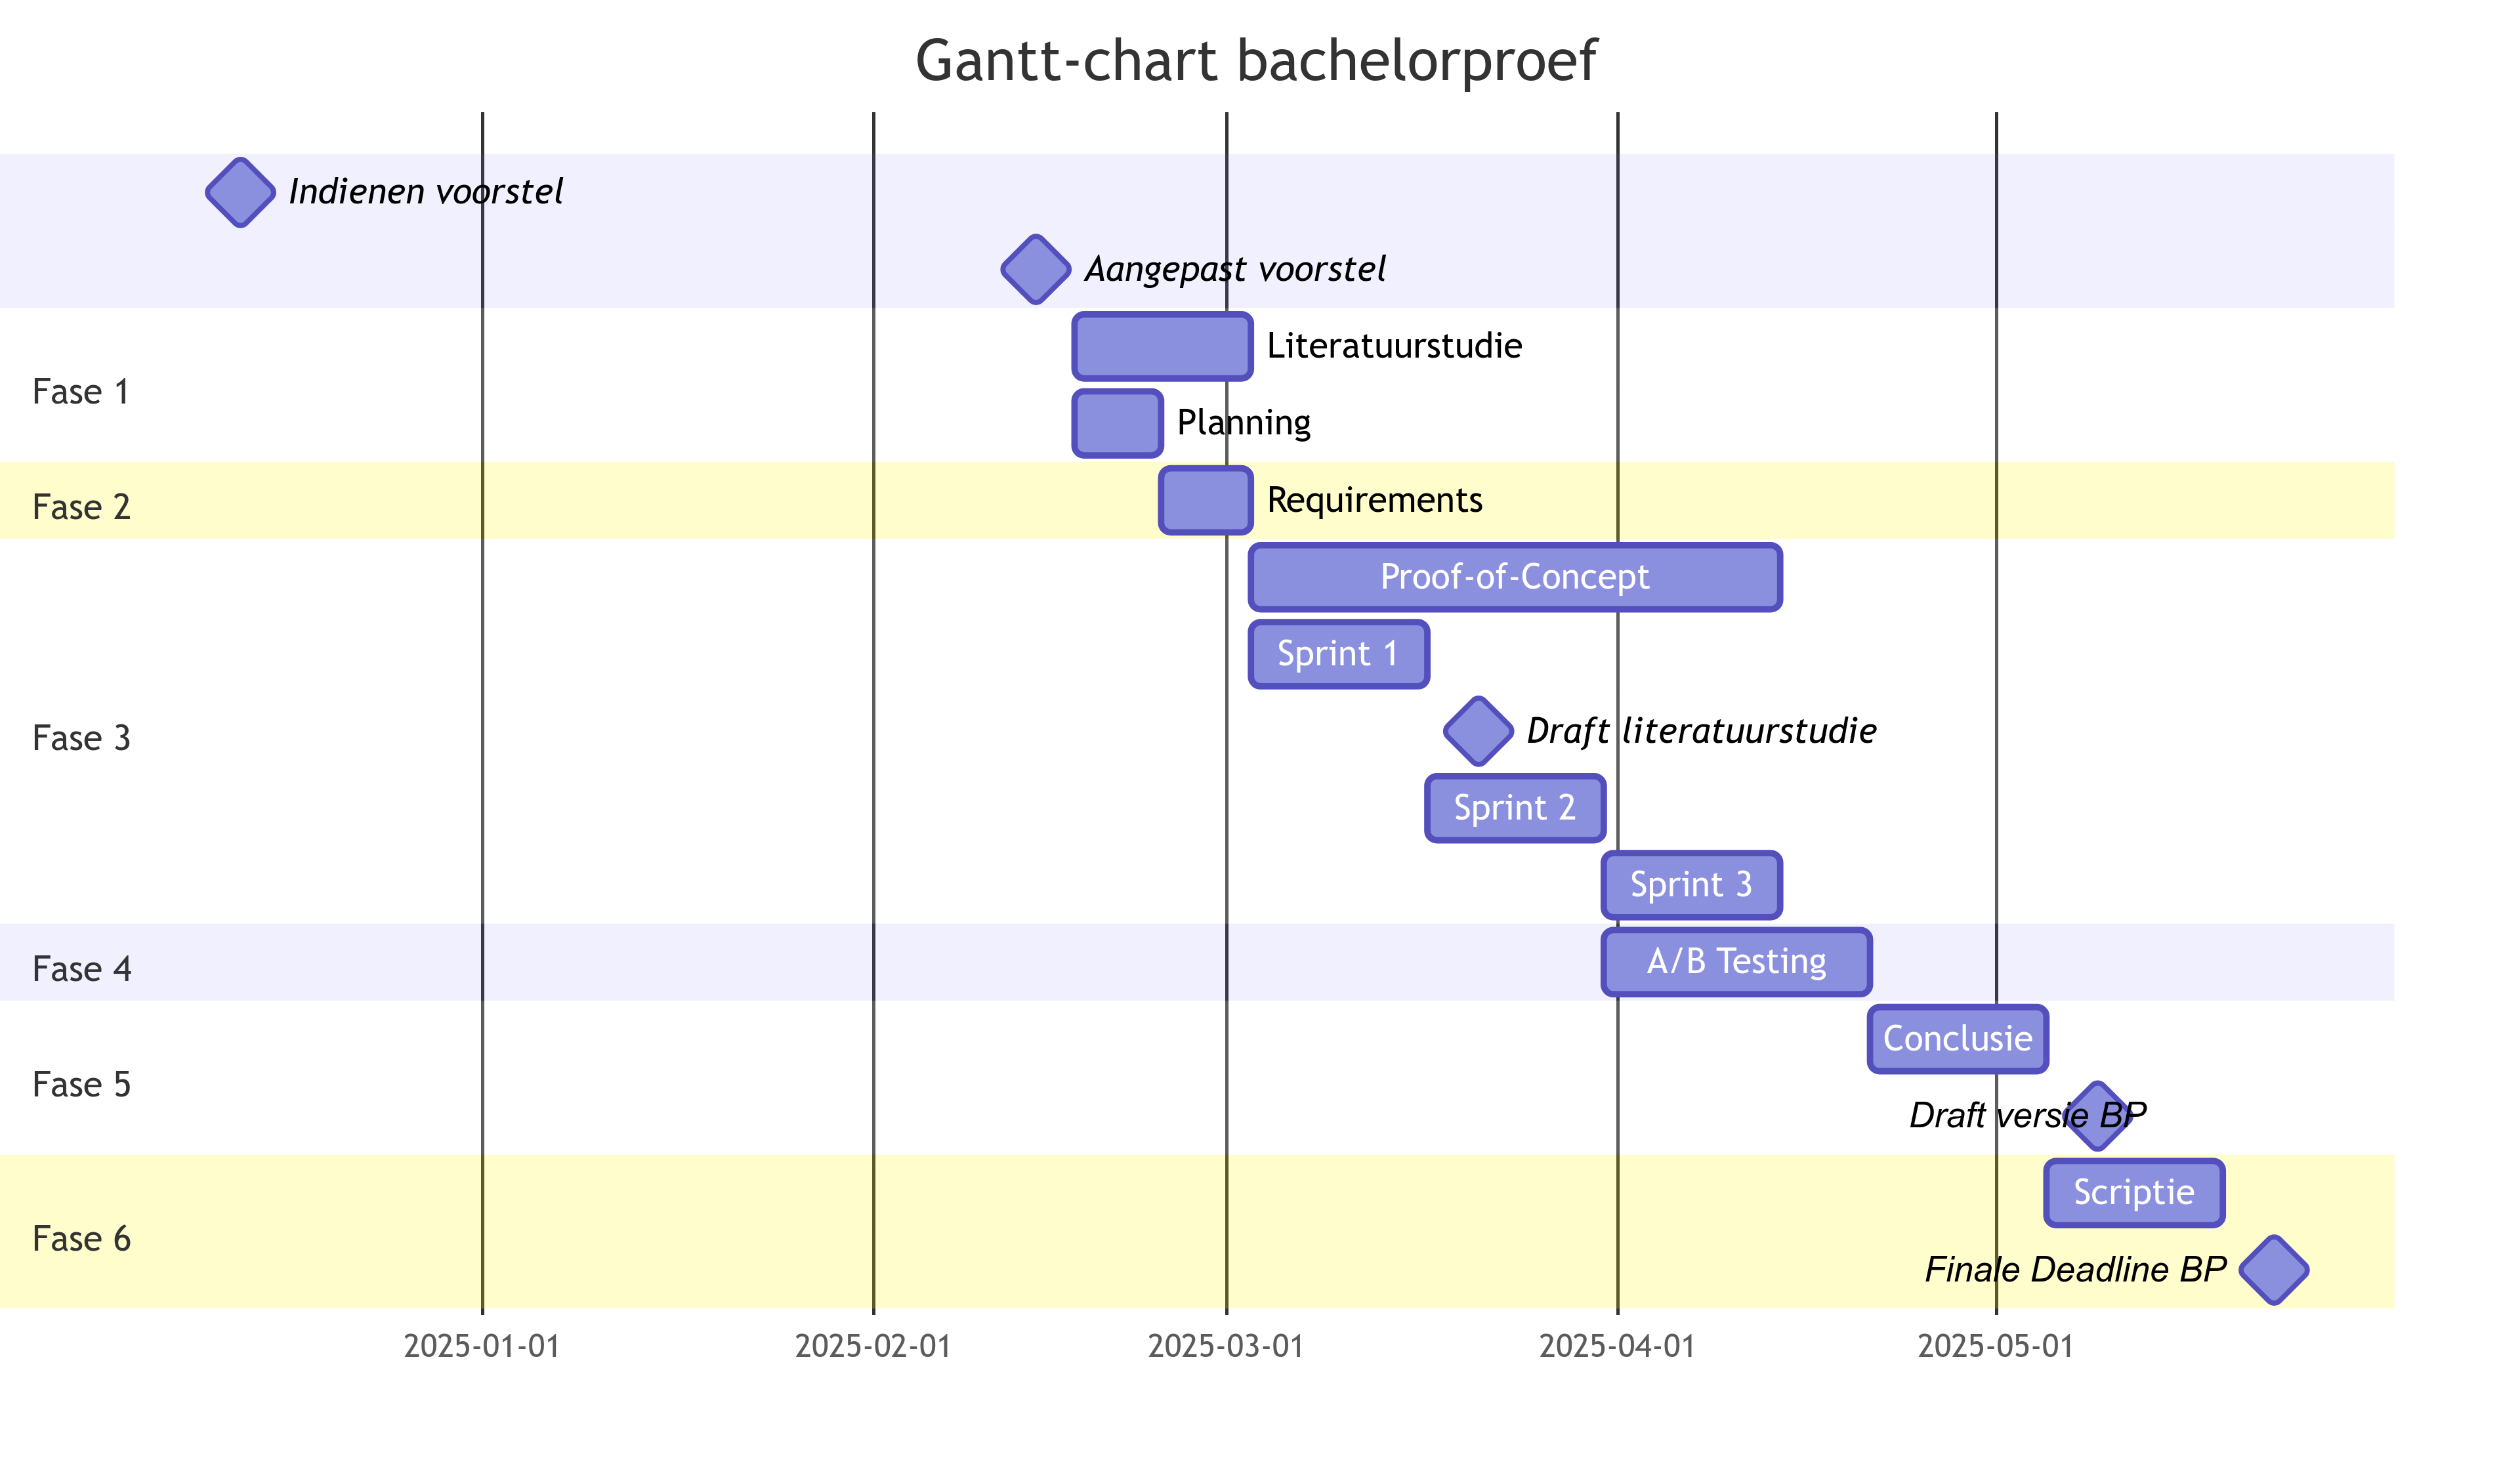
\includegraphics[width=\textwidth]{chart.png}
    \caption{\label{fig:gantt}Gantt diagram met de verschillende fasen en milestones van het onderzoek.}
\end{figure*}

In de vierde fase wordt de pilotversie van de applicatie getest. Tijdens deze fase wordt de applicatie geïmplementeerd binnen een gecontroleerde omgeving, waarbij een beperkte gebruikersgroep toegang krijgt. Deze groep wordt zorgvuldig geselecteerd om een representatieve steekproef van de hele gemeente te vormen. Gedurende de pilotperiode, die drie weken in beslag neemt, zal de focus liggen op het verzamelen van gebruikersdata en het evalueren van de effectiviteit van de geïmplementeerde gamificatie-elementen. Feedback van de gebruikers wordt verzameld via enquêtes en interviews, technische prestatiegegevens worden steeds gemonitord. 

Zoals eerder vermeld is het belangrijk in deze fase om 2 groepen te hebben. Een groep met de gamificatie-elementen en een zonder. Zo kunnen de resultaten van beide groepen vergeleken worden. 

Deze fase biedt de mogelijkheid om eventuele bugs of tekortkomingen in een vroeg stadium te identificeren. Die aanpassingen zullen gerapporteerd worden op het einde van dit onderzoek als richtlijnen voor de verdere ontwikkeling.

De testfase zal beginnen aan de start van sprint drie. De functionaliteiten in de laatste sprint zullen dan getest worden nadien. Alles wat ervoor al af is, kan al getest worden door eindgebruikers.

Vervolgens zal in de vijfde fase de data die verzameld is tijdens de vorige fase grondig geanalyseerd worden. Deze analyse bevat zowel een kwantitatieve als kwalitatieve evaluatie van de verzamelde gegevens. De kwantitatieve data, zoals het aantal keer dat de applicatie gebruikt wordt, success van gamificatie-elementen,... worden geanalyseerd om patronen te herkennen. 

Tegelijkertijd wordt de kwalitatieve feedback van de gebruikers geëvalueerd om inzicht te krijgen in de tekortkomingen die deze applicatie zou bevatten. De bevindingen vormen samen de conclusie van dit onderzoek.

Tot slot, in de zesde en laatste fase, wordt de scriptie van dit onderzoek afgewerkt. Alle resultaten en bevindingen worden overzichtelijk en gestructureerd neergeschreven in dit verslag. Uiteraard is het van belang om in alle fasen de bevindingen bij te houden. Vandaar dat deze fase over alle andere fasen heen loopt. In de laatste twee weken zal er dan tijd zijn om alles aan elkaar te schrijven om een coherent geheel te vormen.

Een overzicht van de verschillende fasen vind je terug in Figuur 1.

\section{Verwachte resultaten}%
\label{sec:verwachte-resultaten}
Uit de studie wordt verwacht dat de implementatie van de gamification-elementen een significante verbetering tonen in de betrokkenheid van de burgers. Dit is gebaseerd op vooraande onderzoeken en theoretische modellen die de effectiviteit van gamification aantonen in vergelijkbare contexten.

Het onderzoek verwacht dat deze verhoogde betrokkenheid zal leiden tot een grotere deelname aan bestaande initiatieven, zoals buurtmoestuinen, deelauto's en de jaarlijkse duurzaamheidsbeurs.

\section{Conclusie}%
\label{sec:discussie-conclusie}

Samenvattend wordt verwacht dat de implementatie van gamification in de gemeente Zonnedorp niet alleen de betrokkenheid van burgers zal verhogen, maar ook zal leiden tot een duurzame gedragsverandering richting een milieuvriendelijker leven. Dit zelfs wanneer er op lange termijn die spelelementen vervallen.  De PoC en de daaropvolgende aanbevelingen zullen dienen als waardevolle bijdragen voor toekomstige toepassingen van gamification in duurzaamheidsinitiatieven van een gemeente.

\printbibliography[heading=bibintoc]

\end{document}